\documentclass[a4paper,12pt]{article}
\usepackage{../../mypackages}
\usepackage{../../macros}

\setlength{\parindent}{0pt}


\begin{document}

\title{Activité}
\author{N. Bancel}
\date{Janvier 2025}
\maketitle

\section*{Enoncé}

\begin{figure}[H]
    \centering
    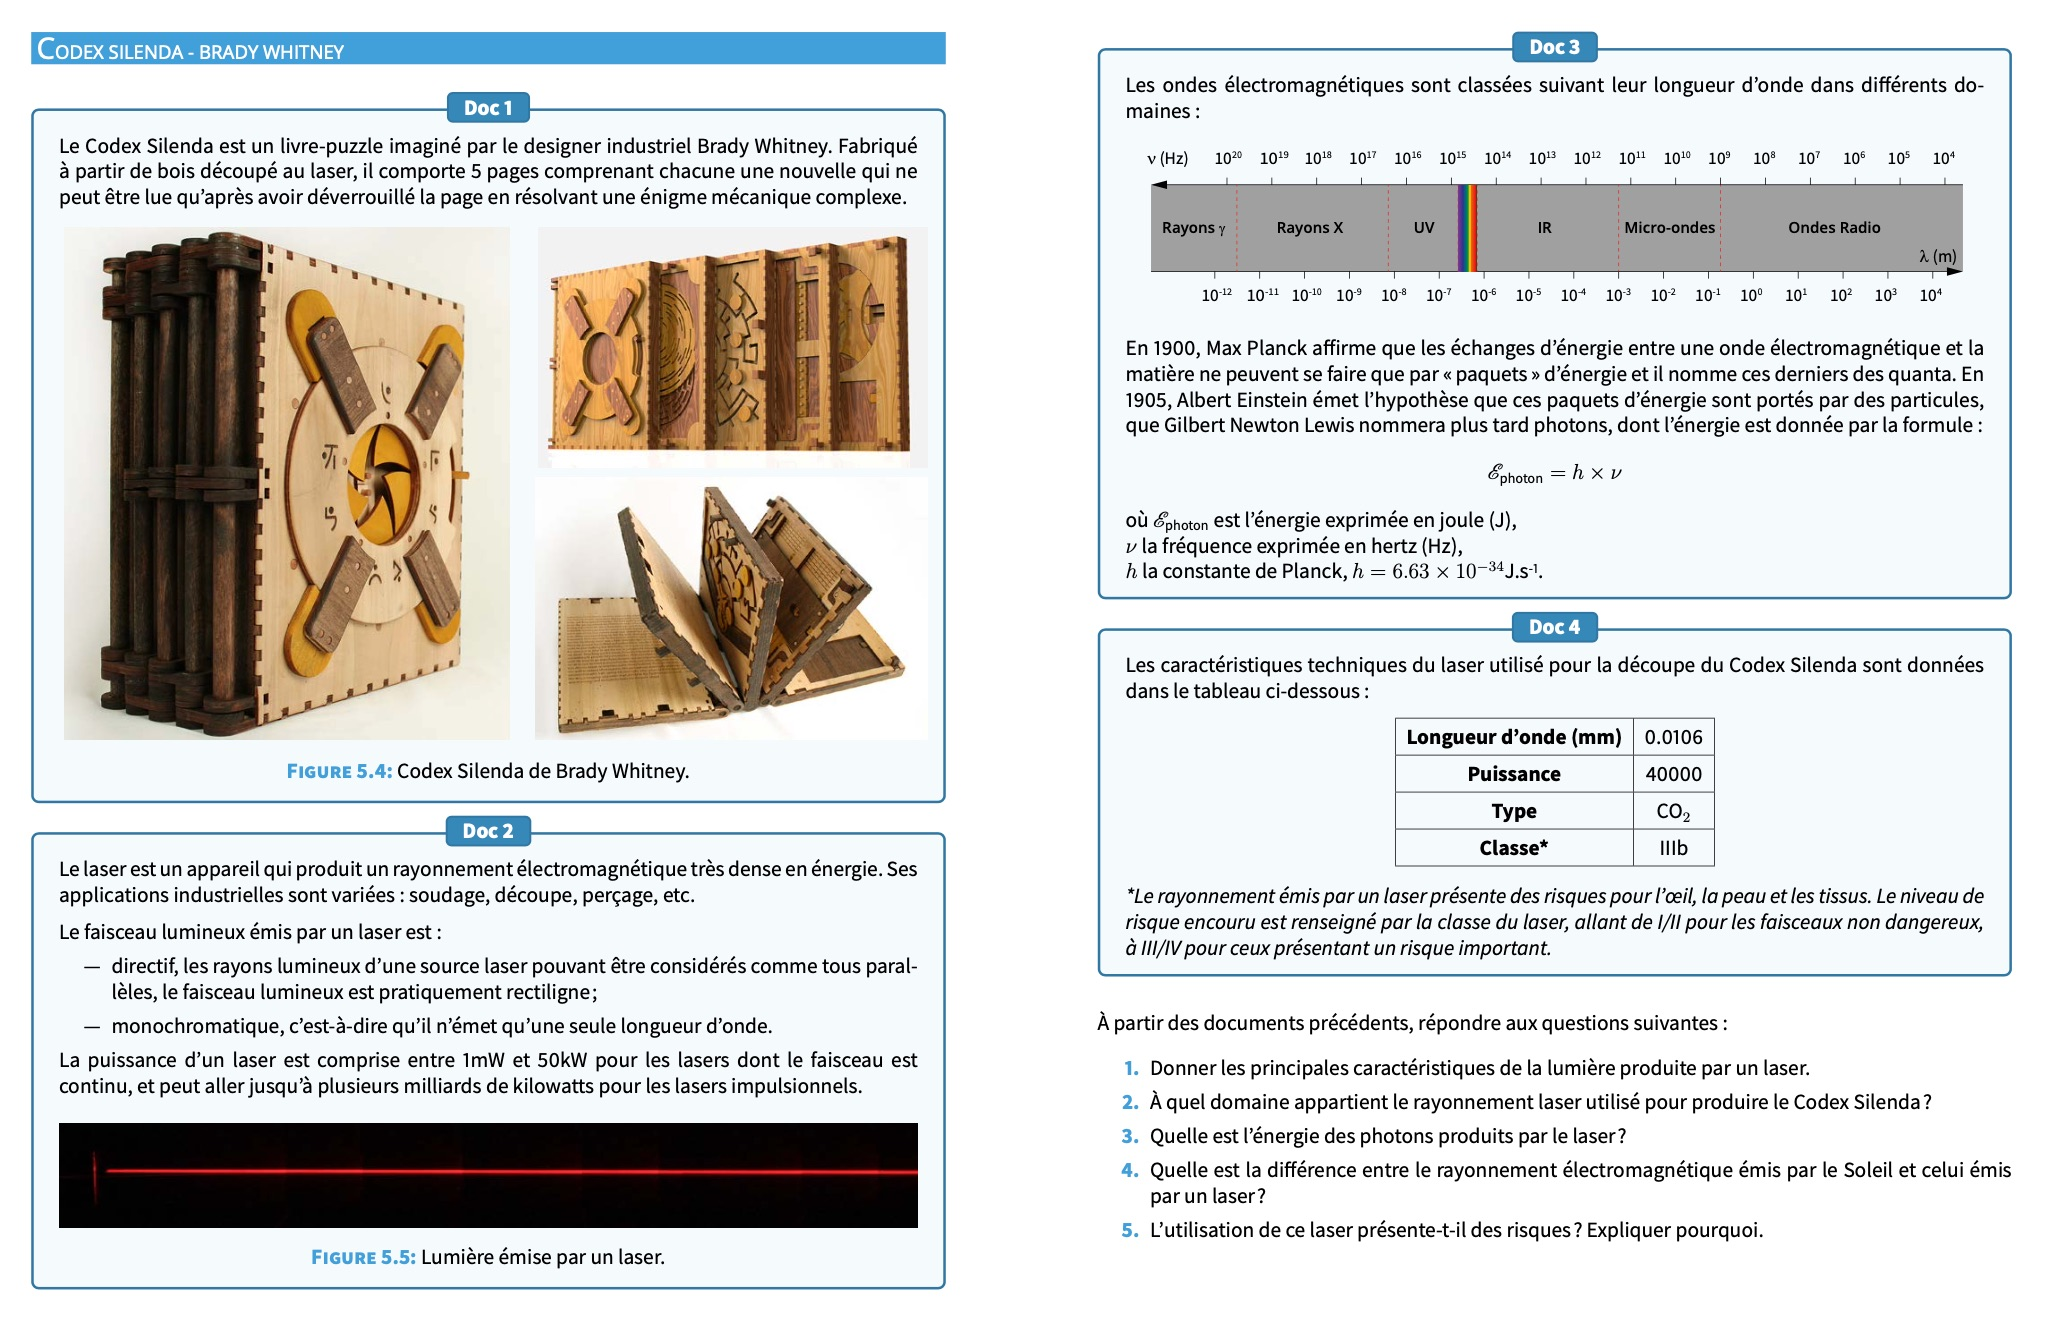
\includegraphics[width=1\linewidth]{activite_lumiere.jpg}
    \captionsetup{labelformat=empty}
    \caption{\label{} Activité 2 page 85}
  \end{figure}

\section*{Correction des questions}

\textbb{Question 1 : Donner les principales caractéristiques de la lumière produite par un laser.}
\vspace{1em}
\begin{itemize}[noitemsep]
    \item La lumière laser est \textbf{directe}, car les rayons lumineux sont pratiquement parallèles.
    \item Elle est \textbf{monochromatique}, c'est-à-dire qu'elle possède une seule longueur d'onde.
    \item Elle est \textbf{cohérente}, ce qui signifie que les ondes lumineuses sont en phase.
\end{itemize}

\textbb{Question 2 : À quel domaine appartient le rayonnement laser utilisé pour produire le Codex Silenda ?} \par
\vspace{1em}
Le laser utilisé appartient au \textbf{domaine infrarouge}, car sa longueur d'onde est de $0,0106$ mm ($10,6 \ \mu m$ : $0,0106 \, \text{mm} = 1,06 \times 10^{-5} \, \text{m}$), ce qui correspond aux longueurs d'onde situées dans l'infrarouge.

\textbb{Question 3 : Quelle est l'énergie des photons produits par le laser ?} \par 
\vspace{1em}

La formule pour l'énergie d'un photon est :
\[ E_{\text{photon}} = h \cdot \nu \]
Avec :
\begin{itemize}
    \item $h = 6,63 \times 10^{-34} \ \text{J} \cdot \text{s}$ (constante de Planck),
    \item $\nu = \frac{c}{\lambda}$, où $c = 3,00 \times 10^{8} \ \text{m/s}$ (vitesse de la lumière) et $\lambda = 0,0106 \ \text{mm} = 1,06 \times 10^{-5} \ \text{m}$ (longueur d'onde).
\end{itemize}

Ainsi :
\[ \nu = \frac{3,00 \times 10^{8}}{1,06 \times 10^{-5}} = 2,83 \times 10^{13} \ \text{Hz} \]
\[ E_{\text{photon}} = 6,63 \times 10^{-34} \cdot 2,83 \times 10^{13} = 1,88 \times 10^{-20} \ \text{J} \]

\textbb{Question 4 : Quelle est la différence entre le rayonnement électromagnétique émis par le Soleil et celui émis par un laser ?}

\begin{itemize}[noitemsep]
    \item Le \textbf{rayonnement solaire} est \textbf{polychromatique}, il contient un large spectre de longueurs d'onde (du rayonnement ultraviolet au rayonnement infrarouge).
    \item Le \textbf{rayonnement laser}, en revanche, est \textbf{monochromatique} (une seule longueur d'onde) et cohérent.
    \item De plus, le rayonnement solaire est diffus alors que le rayonnement laser est direct et concentré.
\end{itemize}

\textbb{Question 5 : L'utilisation de ce laser présente-t-il des risques ? Expliquer pourquoi.}

Oui, l'utilisation de ce laser présente des risques. En effet :
\begin{itemize}[noitemsep]
    \item Le laser est classé \textbf{classe IIIb}, ce qui signifie qu'il peut causer des lésions graves aux yeux et à la peau en cas d'exposition directe.
    \item La forte densité d'énergie du faisceau laser peut également provoquer des brûlures ou des dommages aux tissus.
    \item Par conséquent, il est essentiel de respecter les consignes de sécurité lors de l'utilisation du laser, notamment le port de protections adaptées.
\end{itemize}

\end{document}
